\documentclass[10pt,reqno]{amsart}
\usepackage{amscd,amssymb,amsmath,latexsym,enumerate}
\usepackage{tikz}
\usetikzlibrary{calc}
\usepackage{tikz-cd}
\usepackage{color}
\usepackage{xcolor}

\begin{document}

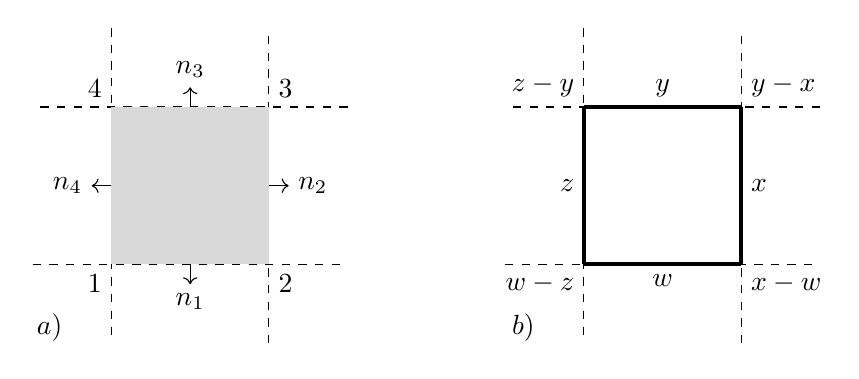
\begin{tikzpicture}
	\begin{scope}[shift={(-3,0)},scale=0.5]
		{
			% Define the square coordinates
			\coordinate (A) at (-2,-2);
			\coordinate (B) at (2,-2);
			\coordinate (C) at (2,2);
			\coordinate (D) at (-2,2);

			% Draw extended lines
			\draw[thin, dashed] ($(A)!-0.5!(B)$) -- ($(B)!-0.5!(A)$);
			\draw[thin, dashed] ($(B)!-0.5!(C)$) -- ($(C)!-0.5!(B)$);
			\draw[thin, dashed] ($(C)!-0.5!(D)$) -- ($(D)!-0.5!(C)$);
			\draw[thin, dashed] ($(D)!-0.5!(A)$) -- ($(A)!-0.5!(D)$);

			% Draw the square and shade it
			\fill[gray!30] (A) -- (B) -- (C) -- (D) -- cycle;

			% Label the outward normals
			\draw[->] (0,-2) -- +(0,-0.5) node[below] {$n_1$};
			\draw[->] (2,0) -- +(0.5,0) node[right] {$n_2$};
			\draw[->] (0,2) -- +(0,0.5) node[above] {$n_3$};
			\draw[->] (-2,0) -- +(-0.5,0) node[left] {$n_4$};

			\draw (A) node[below left] {$1$};
			\draw (B) node[below right] {$2$};
			\draw (C) node[above right] {$3$};
			\draw (D) node[above left] {$4$};


			\draw (-3,-3) node[below left] {$a)$};
		}
	\end{scope}
	\begin{scope}[shift={(3,0)},scale=0.5]
		{
			% Define the square coordinates
			\coordinate (A) at (-2,-2);
			\coordinate (B) at (2,-2);
			\coordinate (C) at (2,2);
			\coordinate (D) at (-2,2);

			% Draw extended lines
			\draw[thin, dashed] ($(A)!-0.5!(B)$) -- ($(B)!-0.5!(A)$);
			\draw[thin, dashed] ($(B)!-0.5!(C)$) -- ($(C)!-0.5!(B)$);
			\draw[thin, dashed] ($(C)!-0.5!(D)$) -- ($(D)!-0.5!(C)$);
			\draw[thin, dashed] ($(D)!-0.5!(A)$) -- ($(A)!-0.5!(D)$);

			% Draw the square and shade it

			\draw[line width=0.5mm] (A) -- (B) {};
			\draw[line width=0.5mm] (B) -- (C) {};
			\draw[line width=0.5mm] (C) -- (D) {};
			\draw[line width=0.5mm] (D) -- (A) {};
			% Label the outward normals
			\draw (0,-2) node[below] {$w$};
			\draw (2,0)  node[right] {$x$};
			\draw (0,2) node[above] {$y$};
			\draw (-2,0)  node[left] {$z$};

			\draw (A) node[below left] {$w-z$};
			\draw (B) node[below right] {$x-w$};
			\draw (C) node[above right] {$y-x$};
			\draw (D) node[above left] {$z-y$};

			\draw (-3,-3) node[below left] {$b)$};
		}
	\end{scope}
\end{tikzpicture}

\end{document}